\documentclass[oneside,a4paper,14pt]{extarticle} %размер шрифта 14
\usepackage[T1,T2A]{fontenc}
\usepackage[a4paper,letterpaper,top=20mm,bottom=20mm,left=20mm,right=10mm]{geometry}
\usepackage[russian]{babel} %поддержка русского языка
\usepackage{textcomp} %текстовые символы
\usepackage{indentfirst} %корректировка отступов
\usepackage{graphicx} %работа с изображениям
\usepackage{mwe} % for blindtext and example-image-a in example
\usepackage{wrapfig}
\usepackage{caption}
\usepackage{amsmath}
\usepackage{amsfonts}
\usepackage{amsthm}
\usepackage[all]{xy}
\usepackage[breaklinks]{hyperref}
\usepackage{titlesec}
\usepackage{listings}
\usepackage{xcolor}

\titleformat{\section}
{\normalsize\bfseries} 
{\thesection} {1em}{} 
\titleformat{\subsection}
{\normalsize\bfseries}
{\thesubsection} {1em}{} 
\titleformat{\subsubsection}
{\normalsize\bfseries}
{\thesubsection} {1em}{}
\definecolor{mygreen}{HTML}{A6E392}
\definecolor{myback}{HTML}{1e1e2e}
\definecolor{mykeyw}{HTML}{cba6f7}
\definecolor{mytext}{HTML}{faa975}
\lstset{
    basicstyle=\small\ttfamily,
    keywordstyle=\color{mykeyw},
    commentstyle=\color{green},
    stringstyle=\color{mygreen},
    numbers=left,
    numberstyle=\tiny,
    stepnumber=1,
    numbersep=10pt,
    tabsize=2,
    breaklines=true,
    language=C
}

\renewcommand\baselinestretch{1.45}\normalsize
\setlength{\parindent}{1.25cm}
\usepackage{indentfirst}


\begin{document}
\newpage\thispagestyle{empty}
\begin{center}
	МИНИСТЕРСТВО НАУКИ И ВЫСШЕГО ОБРАЗОВАНИЯ\\
	РОССИЙСКОЙ ФЕДЕРАЦИИ
	ФЕДЕРАЛЬНОЕ ГОСУДАРСТВЕННОЕ БЮДЖЕТНОЕ\\
	ОБРАЗОВАТЕЛЬНОЕ
	УЧРЕЖДЕНИЕ ВЫСШЕГО ОБРАЗОВАНИЯ\\
	«ВЯТСКИЙ ГОСУДАРСТВЕННЫЙ УНИВЕРСИТЕТ»\\
	Институт математики и информационных систем\\
	Факультет автоматики и вычислительной техники\\
	Кафедра электронных вычислительных машин
\end{center}
\vspace{20mm}

\begin{center}
	Отчёт по лабораторной работе №3\\
	по дисциплине\\
	<<Информатика>>\\
	<<Реализация базовых алгоритмов в системах счисления.>>\\
\end{center}
\vspace{48mm}

Выполнил студент гр. ИВТб-1301-05-00 \hspace{11mm} \rule[-0,5mm]{30mm}{0.15mm}\,/Черкасов А. А./


Проверил доцент кафедры ЭВМ \hfill  \rule[-0,5mm]{30mm}{0.15mm}\,/Коржавина А.С./

\vfill
\begin{center}
	Киров\\
	2024
\end{center}

\section*{Цель}

Цель лабораторной работы: закрепить на практике лекционный материал по теме «Системы счисления», реализовав несколько базовых алгоритмов работы в системах счисления с произвольными основаниями.

\section*{Задания}

\begin{enumerate}
	\item Определить количество нулей в двоичной записи числа. \\
	      \textbf{Формат ввода.} \\
	      Целое неотрицательное число в десятичной системе счисления.\\
	      \textbf{Формат вывода.} \\
	      Количество нулей в двоичной записи числа.\\
	      $$
		      \begin{tabular}{ll}
			      \textbf{Ввод} & \textbf{Вывод} \\
			      \hline
			      16            & 4              \\
			      \hline
			      7             & 0              \\
			      \hline
		      \end{tabular}
	      $$
	\item Определить, какая цифра, 0 или 1, стоит в разряде N в двоичной записи числа. \\
	      \textbf{Формат ввода.} \\
	      Через пробел: целое неотрицательное число в десятичной системе счисления и номер разряда в двоичной записи числа.\\
	      \textbf{Формат вывода.} \\
	      Двоичная цифра в разряде номер N.\\
	      $$
		      \begin{tabular}{ll}
			      \textbf{Ввод} & \textbf{Вывод} \\
			      \hline
			      9 1           & 0              \\
			      \hline
			      11 0          & 1              \\
			      \hline
		      \end{tabular}
	      $$
	      \pagebreak
	\item Перевести вещественное число X из системы счисления с основанием K. Перевести число в систему счисления с основанием M. \\
	      \textbf{Формат ввода.} \\
	      В одну строку через пробел 3 числа: вещественное число X, Целое число K из диапазона 2 .. 10, целое число M из диапазона 2 .. 10.\\
	      \textbf{Формат вывода.} \\
	      Вещественное число в системе счисления с основанием M. Количество знаков дробной части определять исходя из количества знаков исходного числа.\\
	      $$
		      \begin{tabular}{ll}
			      \textbf{Ввод} & \textbf{Вывод} \\
			      \hline
			      9.5 10 2      & 1001.1         \\
			      \hline
			      12.1 3 5      & 10.1           \\
			      \hline
		      \end{tabular}
	      $$
	\item Вывести результат выполнения операции (a+b) в системе остаточных классов с N основаниями p1, p2, ..., pN. В случае, если результат выходит за границы диапазона представления чисел, вывести -1, иначе вывести результат в десятичной системе счисления. \\
	      \textbf{Формат ввода.} \\
	      В строке через пробел число модулей N, модули, цифры числа a, цифры числа~b.\\
	      \textbf{Формат вывода.} \\
	      Результат в десятичной системе счисления либо «-1», если результат выходит за границы диапазона.\\
	      $$
		      \begin{tabular}{ll}
			      \textbf{Ввод}       & \textbf{Вывод} \\
			      \hline
			      3 2 3 5 1 1 1 0 2 2 & 3              \\
			      \hline
			      3 2 3 5 0 2 0 0 2 0 & -1             \\
			      \hline
		      \end{tabular}
	      $$
\end{enumerate}
\pagebreak
\section*{Решение}
\begin{figure}[h!]
	\centering
	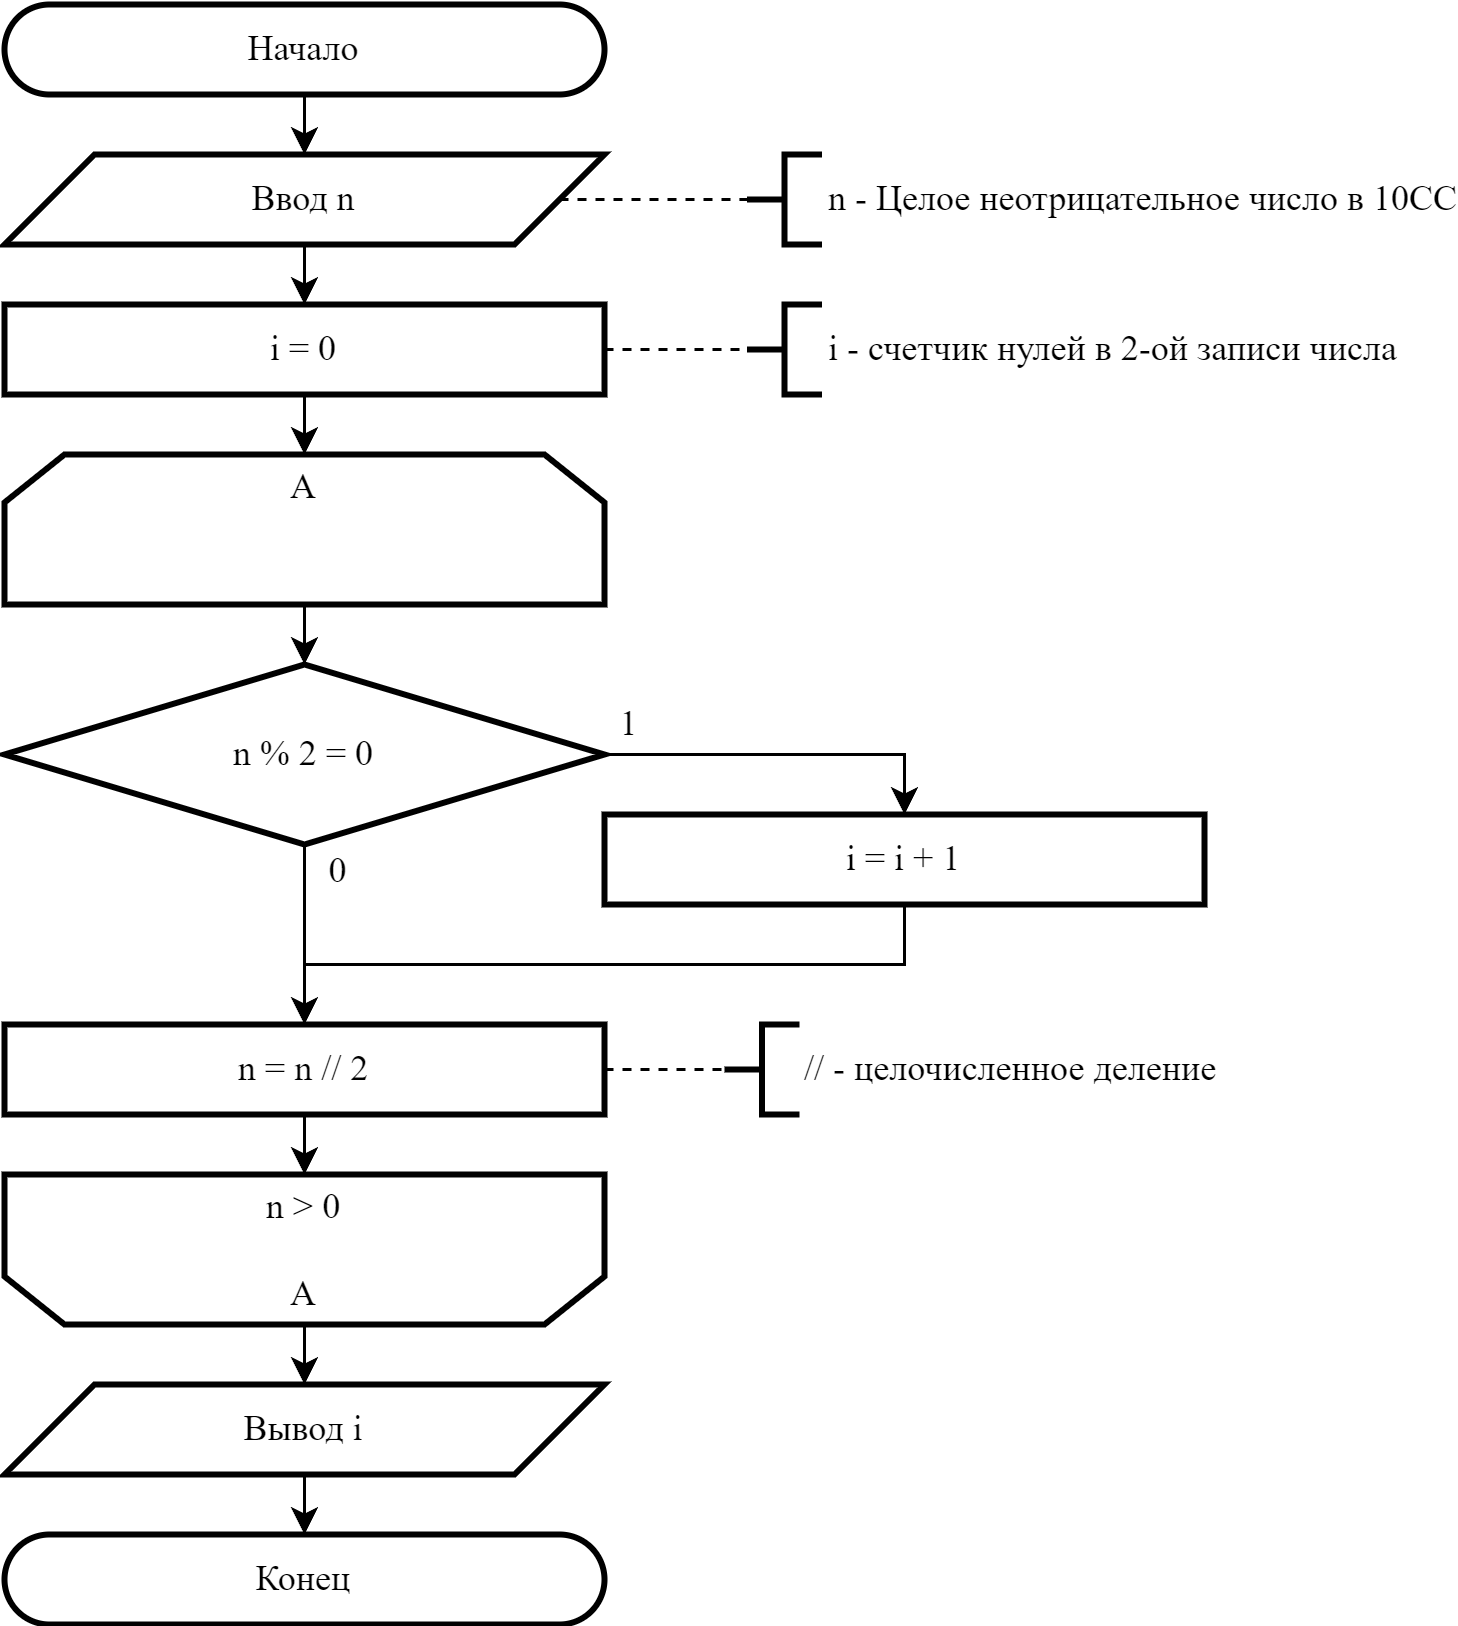
\includegraphics[width=0.8\textwidth]{pics/1-flowchart.png}
	\caption{Схема алгоритма задания 1.}
\end{figure}
\newpage
\begin{figure}[h!]
	\centering
	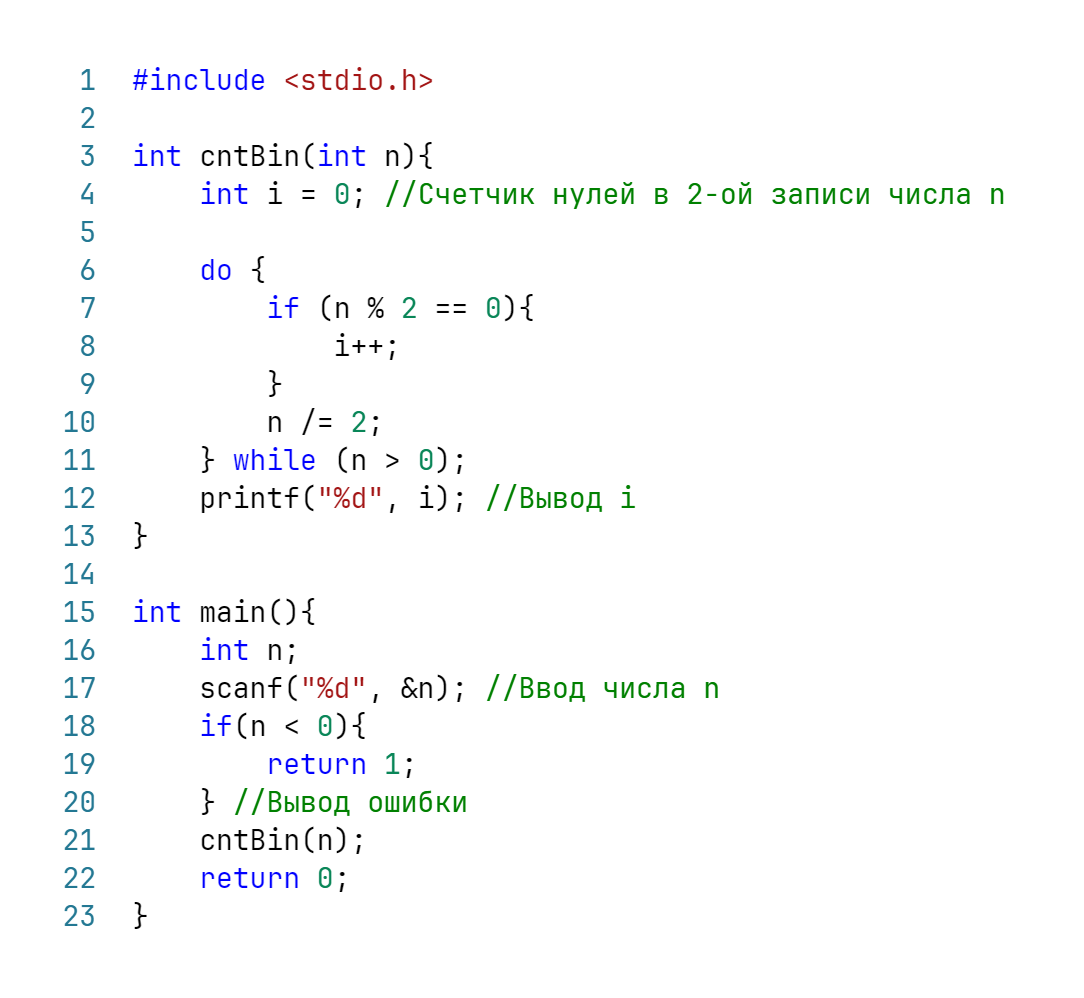
\includegraphics[width=1\textwidth]{pics/1-listing.png}
	\caption*{Листинг 1: Решение задания 1 на языке C}
\end{figure}
\newpage
\begin{figure}[h!]
	\centering
	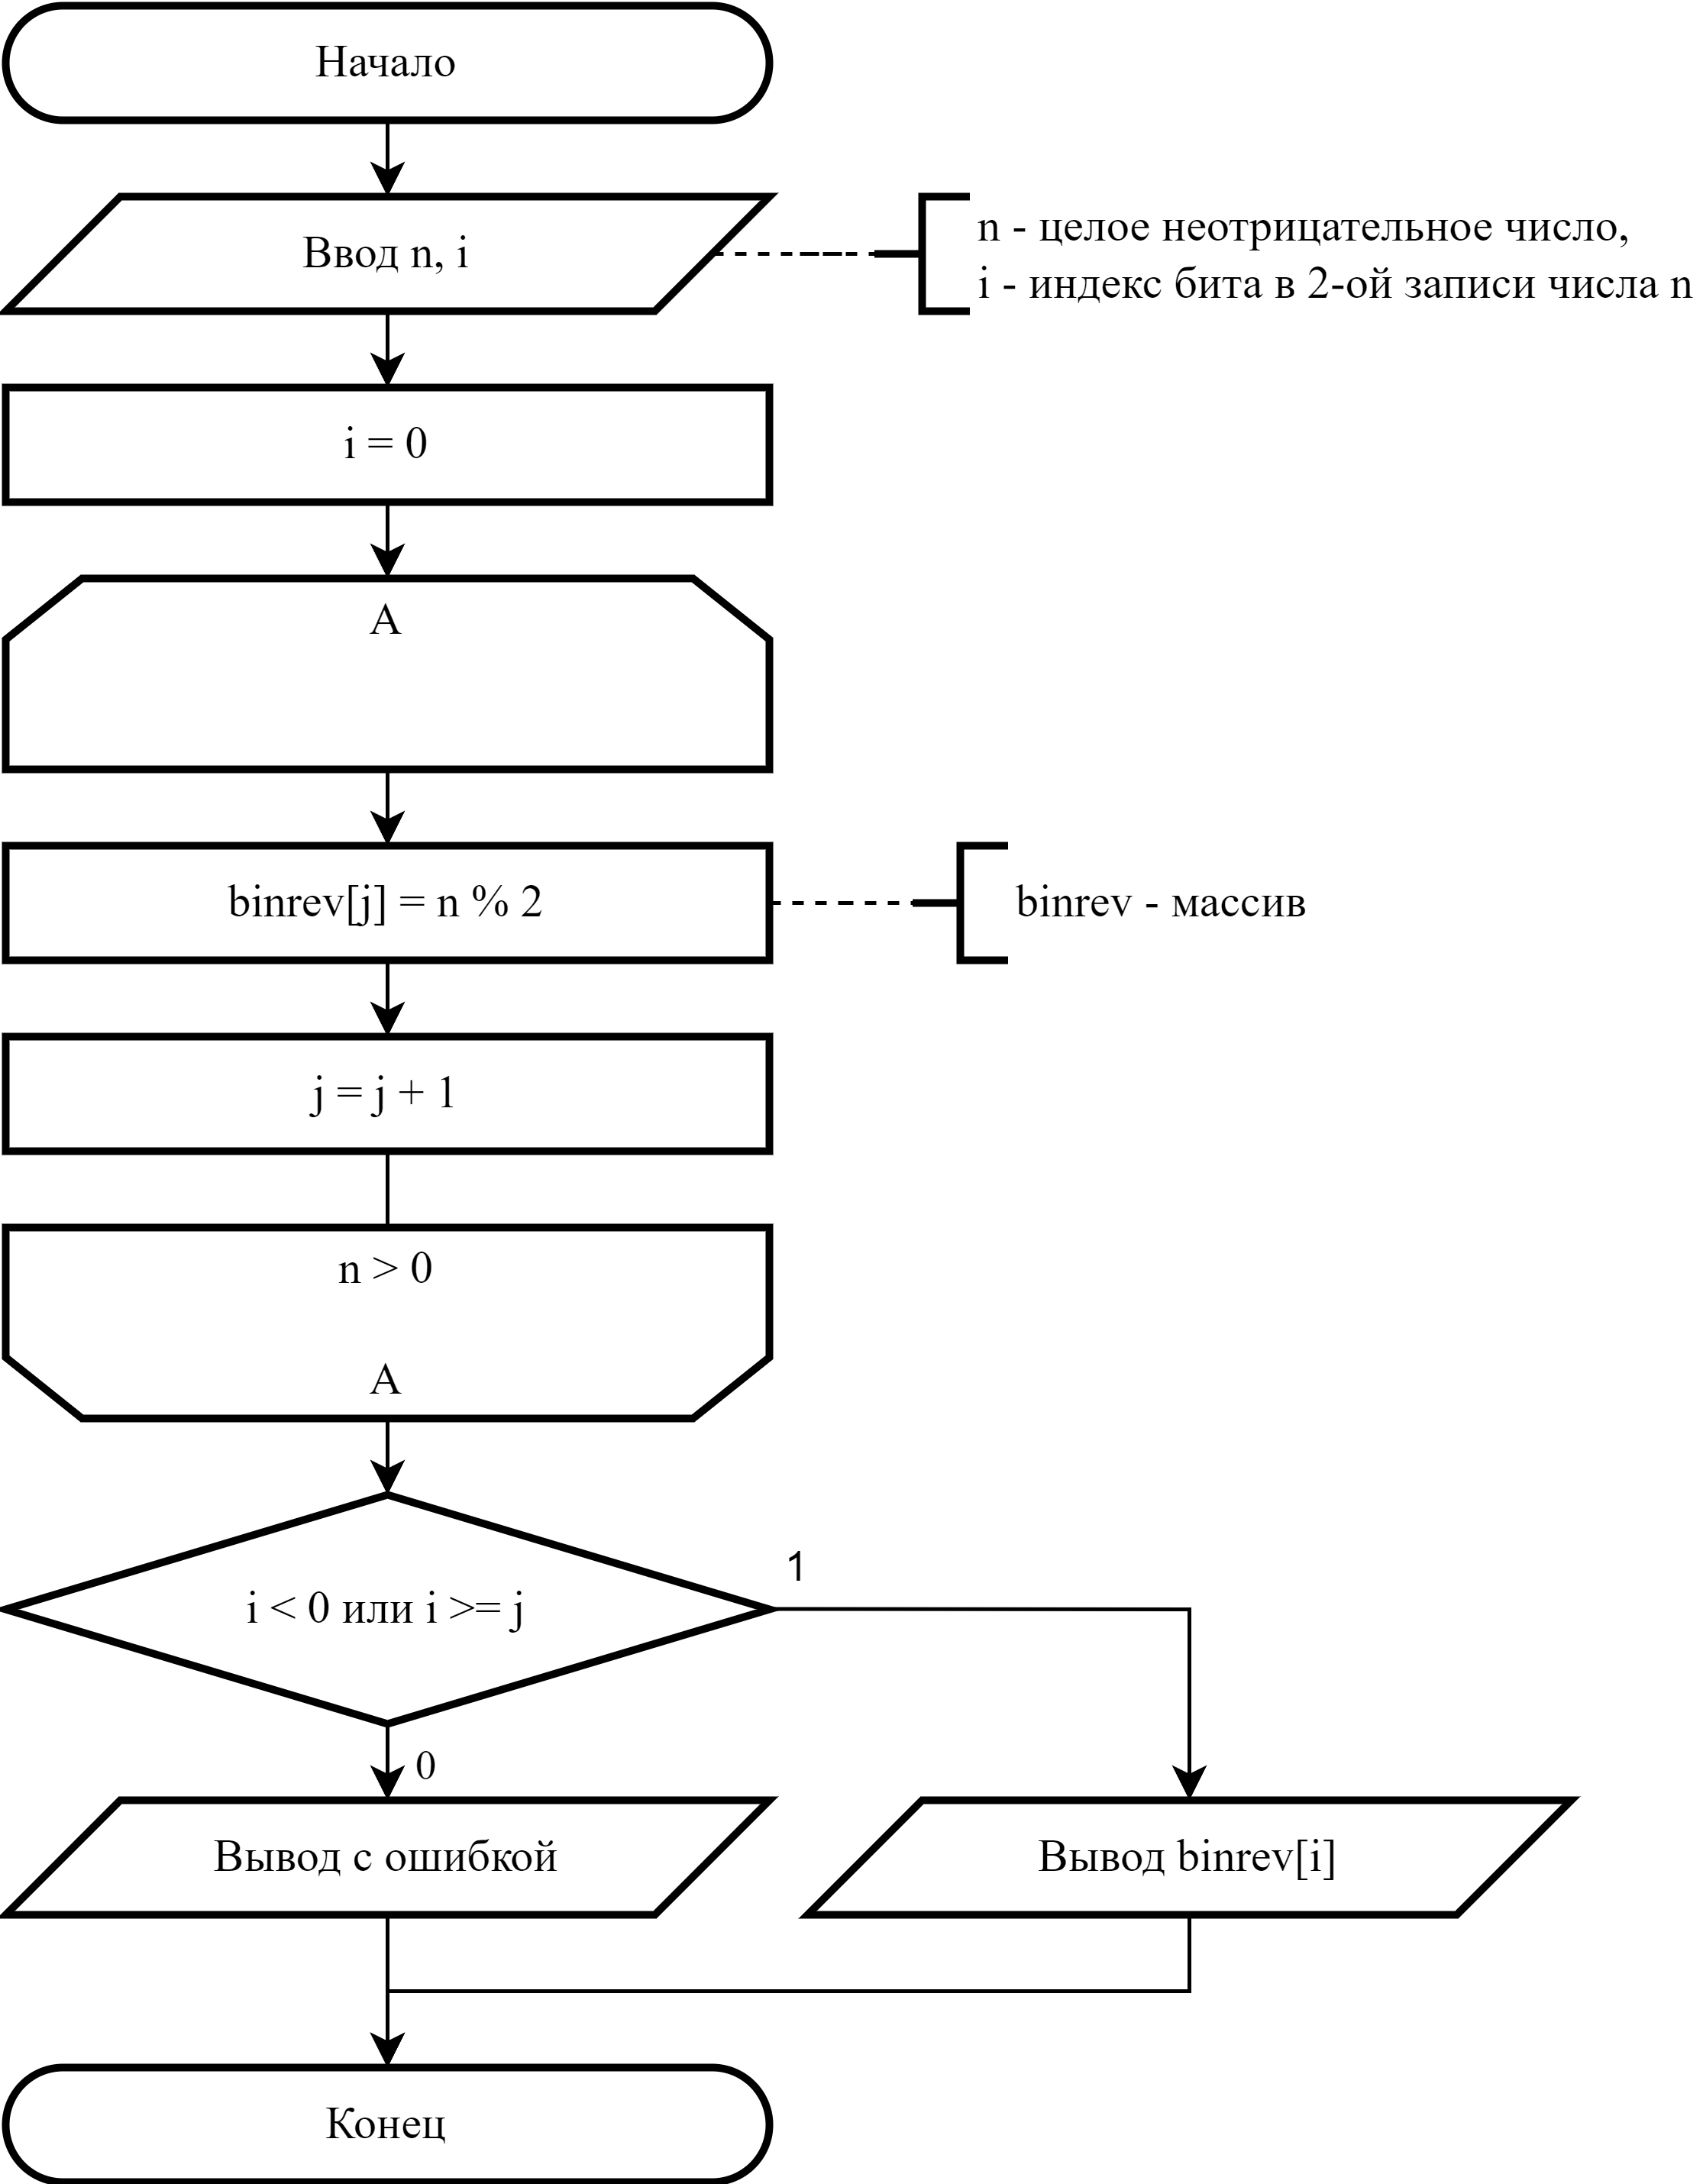
\includegraphics[width=0.8\textwidth]{pics/2-flowchart.png}
	\caption{Схема алгоритма задания 2.}
\end{figure}
\newpage
\begin{figure}[h!]
	\centering
	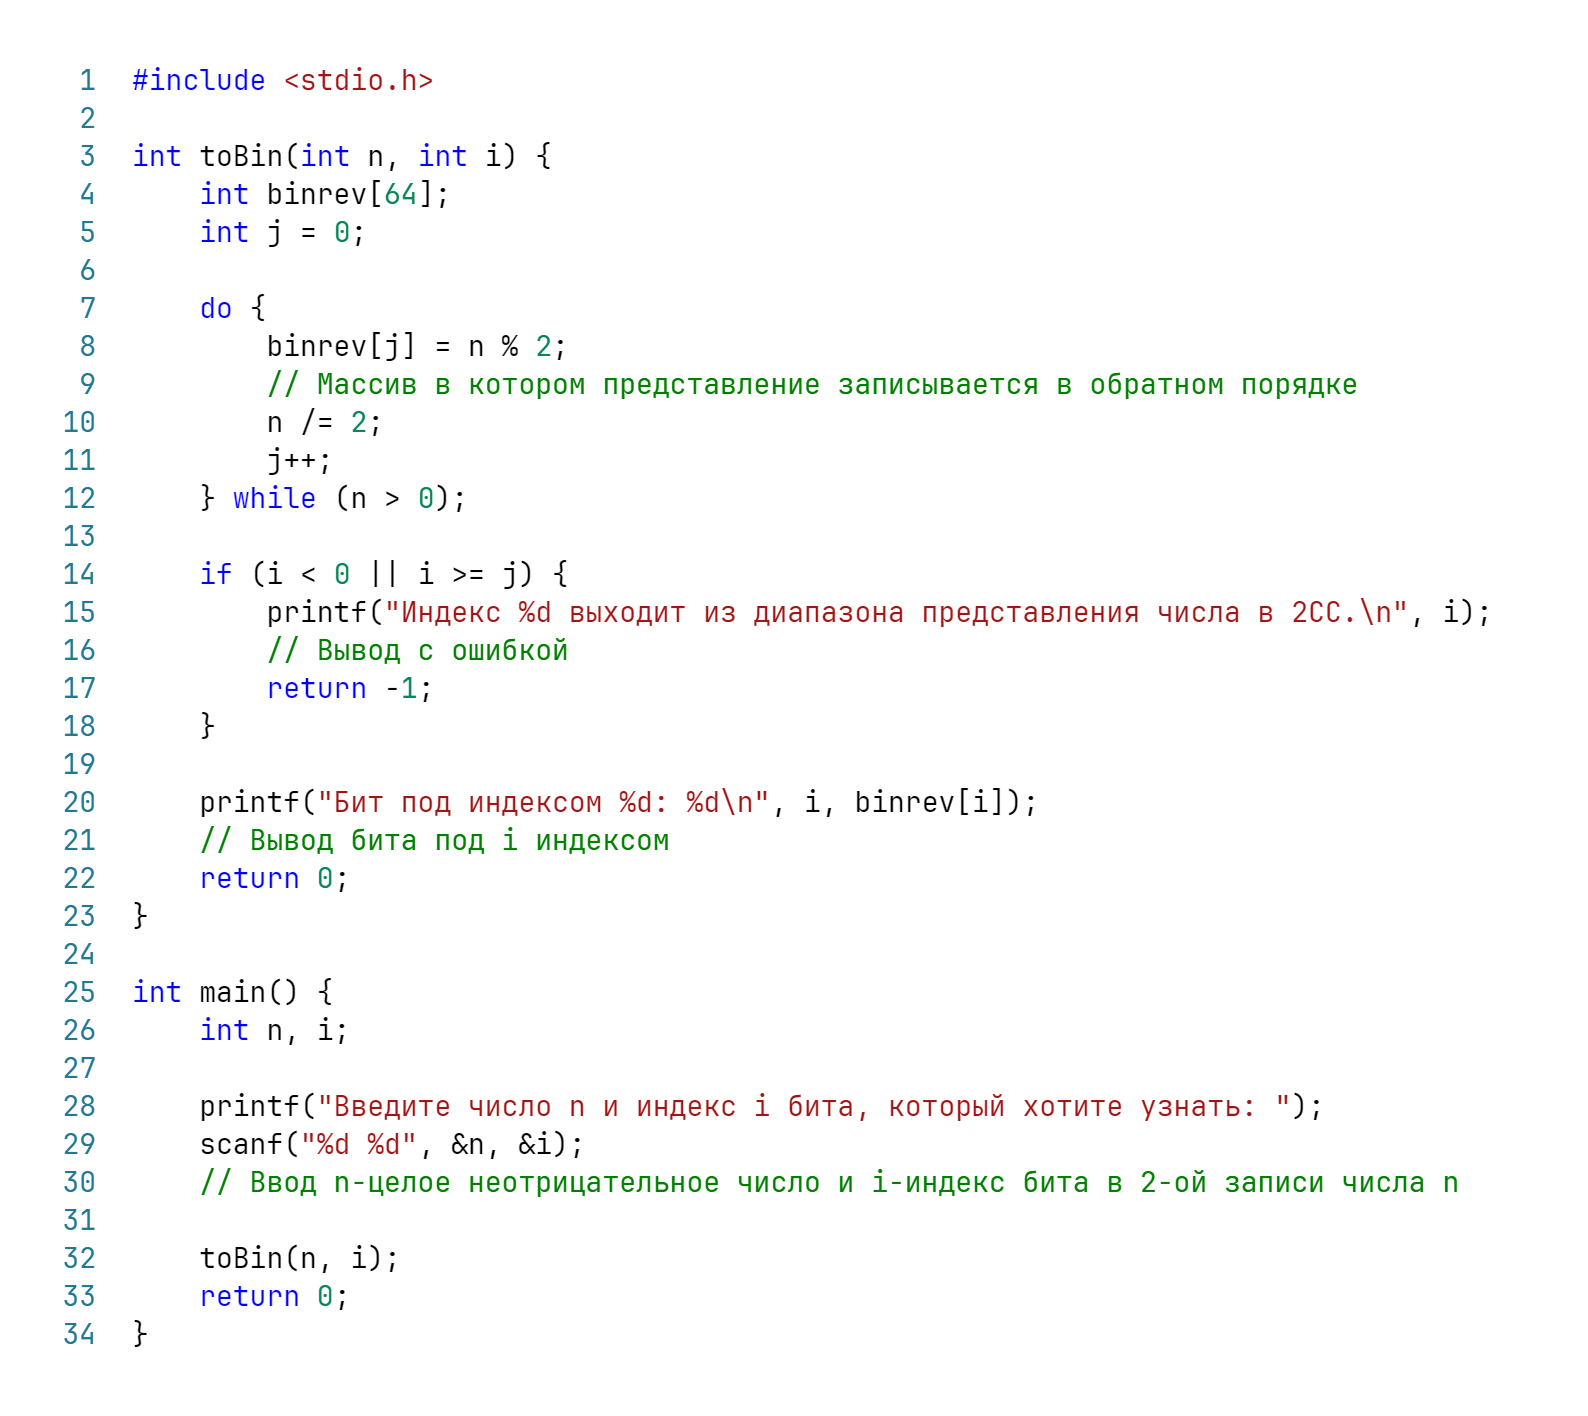
\includegraphics[width=1\textwidth]{pics/2-listing.png}
	\caption*{Листинг 2: Схема алгоритма задания 2.}
\end{figure}
\newpage
\section*{Вывод}
\end{document}